%
% kreisbogen.tex -- Kreisbogen mit zwei verschiedenen Parametrisierungen
%
% (c) 2017 Prof Dr Andreas Müller, Hochschule Rapperswil
%
\documentclass[tikz]{standalone}
\usepackage{times}
\usepackage{txfonts}
\usepackage{pgfplots}
\usepackage{csvsimple}
\usetikzlibrary{arrows,intersections}
\begin{document}
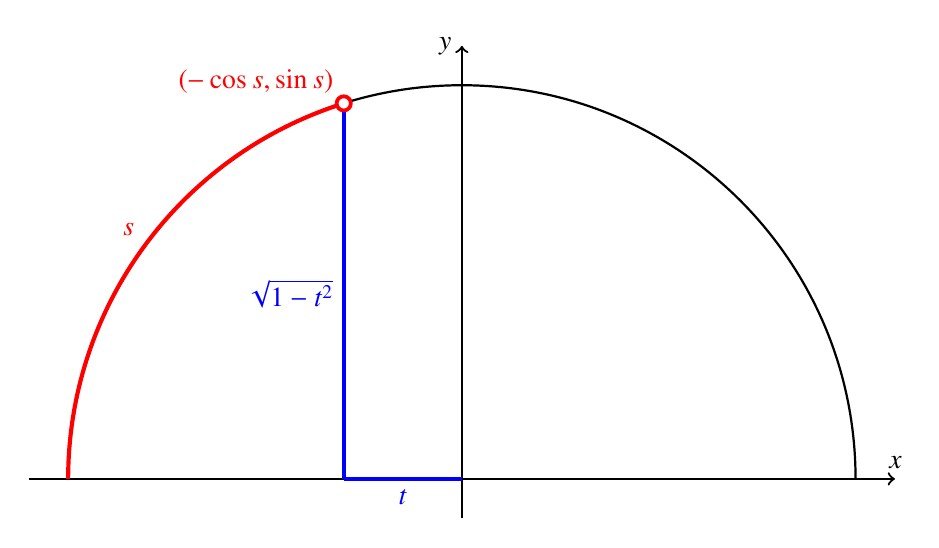
\begin{tikzpicture}[thick,scale=5]
\coordinate (O) at (0,0);

\draw[->] (-1.1,0)--(1.1,0) coordinate[label={above:$x$}];
\draw[->] (0,-0.1)--(0,1.1) coordinate[label={left:$y$}];

\draw[blue,line width=1.5] (-0.3,0)--(-0.3,0.95934);
\draw[blue,line width=1.5] (0,0)--(-0.3,0);

\node at (-0.15,0) [below,blue] {$t$};
\node at (-0.3,0.47) [left,blue] {$\sqrt{1-t^2}$};

\draw (1,0) arc(0:180:1);
\draw[red,line width=1.5] (107.46:1) arc(107.46:180:1);

\node at (143.73:1) [above left,red] {$s$};
\node at (107.46:1) [above left,red] {$(-\cos s,\sin s)$};

\draw[red,fill=red] (107.46:1) circle[radius=0.02] {};
\draw[red,fill=white] (107.46:1) circle[radius=0.016] {};


%\draw[blue,line width=1.5] (-2,0)--(3,2.5);
%
%\draw[->] (-2.55, 0   )--(3.05,  0   ) coordinate[label = {below:$t$}];
%\draw[->] ( 0,   -0.05)--(0   ,  3.05) coordinate[label = {right:$a(t)$}];
%
%\node at ( 0,0) [below right] {$t_0$};
%\node at (-2,0) [below] {$\displaystyle -\frac1{H_0}$};
%\node at (-1.333,0) [below] {$\displaystyle -\frac2{3H_0}$};
%
%\draw (-2,-0.03)--(-2,0.03);
%\draw (-1.3333,-0.03)--(-1.3333,0.03);
%
%\node at (3.05,2.1) [below left] {$\Lambda=0$};
%\node at (2.10,2.85) [above left] {$\Lambda=1$};

\end{tikzpicture}
\end{document}


